\subsection{Cost Category 70: Annualized O\&M Cost (AOC)}

The Operations and Maintenance (O\&M) costs was previously estimated to be 2 \% of the direct cost, assessed annually.  The O\&M cost depends on the system complexity and the requirements of regulations, security and maintenance. The costs are computed based on look-up tables, such as the one shown in Fig. \ref{fig:statista} at 60 USD per kilowatt-year.  

\begin{figure}[b!] 
\centering 
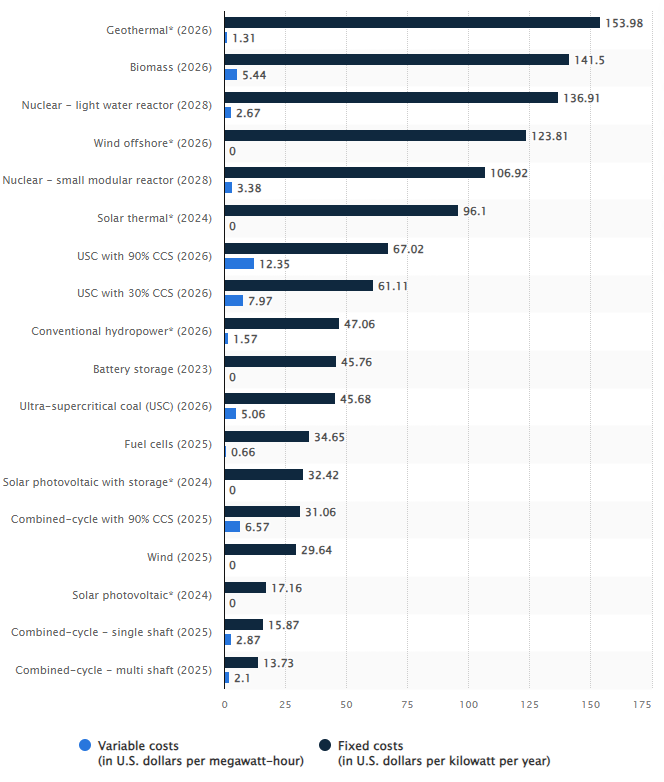
\includegraphics[scale=0.5]{StandardFigures/statista.png} 
\caption{Operations and Maintenance costs for various kinds of power plants.} 
\label{fig:statista} 
\end{figure} 

\begin{verbatim} 
C_OM = 60 * PE * 1000 = C700000  
\end{verbatim} 

Annualized O\&M costs are \$ C700000 M.

\subsubsection*{Cost Category 71 – O\&M Staff}
This Cost Category includes salary costs of O\&M staff.

\subsubsection*{Cost Category 72 – Management Staff}
This Cost Category includes salary costs of operations management staff.

\subsubsection*{Cost Category 73 – Salary-Related Costs}
This Cost Category includes taxes, insurance, fringes, benefits, and any other annual salary-related costs.

\subsubsection*{Cost Category 74 – Operations Chemicals, and Lubricants}

\subsubsection*{Cost Category 75 – Spare Parts}
Cost of any operational spare parts, excluding capital plant upgrades or major equipment that will be capitalized or amortized over some period or quantity of product.\\

Annual Scheduled Replacement Cost. The cost of scheduled component replacement is now included in the annual operations and maintenance charge.  Here we assume that the components in the first wall and the blanket are replaced every 10 years, giving an annual replacement cost of \$ C750000 M.


\subsubsection*{Cost Category 76 – Utilities, Supplies, and Consumables}
Cost of water, gas, electricity, tools, machinery, maintenance equipment, office supplies and similar items purchased annually.

\subsubsection*{Cost Category 77 – Capital Plant Upgrades}
Upgrades to maintain or improve plant capacity, meet future regulatory requirements or plant life extensions.

\subsubsection*{Cost Category 78 – Taxes and Insurance}
Property taxes and insurance costs, excluding salary related.

\subsubsection*{Cost Category 79 – Contingency on Annualized O\&M Costs}
This Cost Category includes an assessment of additional cost necessary to achieve the desired confidence level for the annualized O\&M costs not to be exceeded.
